\chapter{Experiments and Results}

\section{Experimental Setup}

The experimental setup includes the selection of appropriate datasets, splitting the data into training
and testing sets, and tuning hyperparameters for each model.


\begin{lstlisting}[language=Python,caption={Data set fetching using Pandas},label={code:data}]
    J1 = df[df['Junction']==1]
    J2 = df[df['Junction']==2]
    J3 = df[df['Junction']==3]
    J4 = df[df['Junction']==4]
    vehciles_at_J1 = J1['Vehicles']
    vehciles_at_J2 = J2['Vehicles']
    vehciles_at_J3 = J3['Vehicles']
    vehciles_at_J3 = J3['Vehicles']
\end{lstlisting}

\begin{lstlisting}[language=Bash,caption={Sample Result},label={code:confusion matrix}]
    #save
    #logic take input for first 5 hours and
    # predict 6th hour
    # [[1],[2],[3],[4],[5]] [6]
    # [[2],[3],[4],[5],[6]] [7]
    # [[3],[4],[5],[6],[7]] [8]
    def df_to_X_y(df, window_size=5):
    df_as_np = df.to_numpy()
    X =[]
    y = []
    for i in range(len(df_as_np)-window_size):
    row = [[a] for a in
    X.append(row)
    label = df_as_np[i+window_size]
    y.append(label)
    return np.array(X), np.array(y)
\end{lstlisting}

\clearpage

\section{Performance Metrics}

Performance metrics used to evaluate the models include Mean Absolute Error (MAE), Mean Squared Error (MSE), and R-squared (R\textsuperscript{2}).


\begin{lstlisting}[language=Python,caption={Performance Metrics},label={code:data}]
    model1 = Sequential()
    model1.add(LSTM(64, input_shape=(WINDOW_SIZE, 1)))
    model1.add(Dense(8, 'relu'))
    model1.add(Dense(1))
    model1.compile(loss=MeanSquaredError(), optimizer=Adam(learning_rate=0.001), metrics=[RootMeanSquaredError()])
    model1.summary()
\end{lstlisting}




\section{Results and Analysis}

The results of the experiments are analyzed to compare the performance of different models and identify the most effective approaches for traffic flow prediction.

\begin{lstlisting}[language=Python,caption={Performance Metrics},label={code:data}]
    from tensorflow.keras.models import load_model
    model1 = load_model('model1/')
    train_results['Train Predictions'][:150].plot()
    train_results['Train Actual'][:150].plot()
\end{lstlisting}



\begin{figure}[h!]
    \centering
    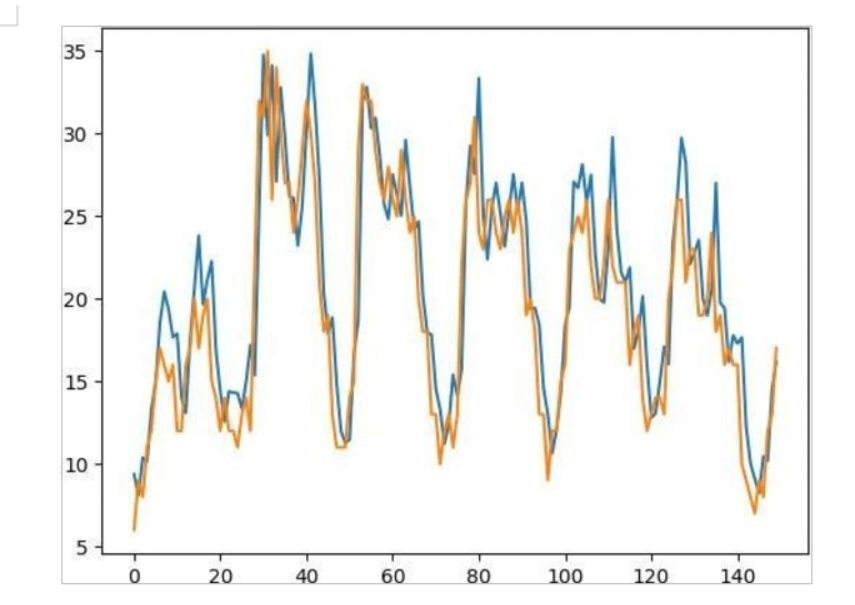
\includegraphics[width=\textwidth]{result2.png}
\end{figure}


\begin{lstlisting}[language=Python,caption={Performance Metrics},label={code:data}]
    val_predictions = model1.predict(X_val).flatten()
    val_results = pd.DataFrame(data={'Validation Predictions':val_predictions, 'Validation Actual':y_val})
    val_results
    val_results['Validation Predictions'][:150].plot()
    val_results['Validation Actual'][:150].plot()
\end{lstlisting}

\begin{figure}[h!]
    \centering
    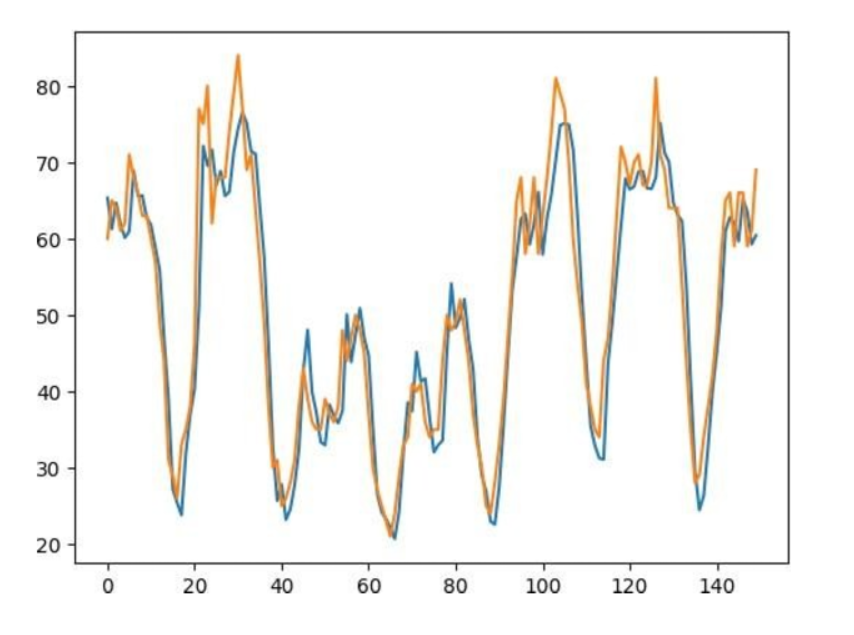
\includegraphics[width=\textwidth]{result_1.png}
\end{figure}
